\documentclass[12pt,
border=1pt]{standalone}
\usepackage{pgfplots}
\usepackage{amsmath}
\usepackage{amssymb}

\pgfplotsset{compat=newest,
	width=6cm, height=5cm,
	xtick pos=left, ytick pos=left
	%            scaled x ticks=real:1e-6,
}
% Kernel 2 FP64
\begin{document}
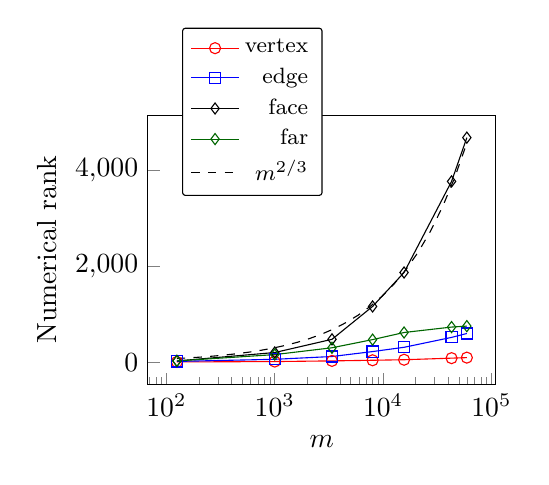
\begin{tikzpicture}
	\begin{axis}[	xlabel={$m$},
	ylabel={Numerical rank},
%		legend pos=south east,
		legend style={
                at={(0.3,0.7)},
               anchor=south,
               legend columns=1,
               cells={anchor=east},
              font=\footnotesize,
               rounded corners=1pt,
               },
		xmode = log,
	   % ymode = log,
		]
		\addplot[
		color=red,
		mark=o,
		] coordinates {
		(125,4	)
		(1000,12	)
		(3375,26	)
		(8000,39	)
		(15625,50	)
		(42875,83	)
		(59319,94)
		};
		\addplot[
		color=blue,
		mark=square,
		] coordinates {
        (125,15	)
		(1000,59)
		(3375,117	)
		(8000,220	)
		(15625,309	)
		(42875,	515)
		(59319,	596)
		};
		\addplot[
		color=black,
		mark=diamond,
		] coordinates {
        (125,25	)
		(1000,200	)
		(3375,475	)
		(8000,1159	)
		(15625,1866	)
		(42875,3762	)
		(59319,4673)
		};
		\addplot[
		color=black!60!green,
		mark=diamond,
		] coordinates {
        (125,25	)
		(1000,157	)
		(3375,299	)
		(8000,469	)
		(15625,617	)
		(42875,730	)
		(59319,750)
		};
		\addplot[mark=none, black, dashed][
		color=black,
		domain = 125:59319,
		] {(3*pow(x,(2/3)};
		\legend{vertex, edge, face, far, $m^{2/3}$}
	\end{axis}
\end{tikzpicture}
\end{document}